\chapterA{Diseño combinacional avanzado}
\section{Módulos combinacionales}

\subsection{Decodificador}
Circuito combinacional con n entradas y $2^{n}$ salidas. Cada salida es uno de los minterms que pueden generarse con n variables.
\[
	D_{i} =\left\{ \begin{array}{l}
		1\; si\; A=i donde\; A= \sum^{n-1}_{j=0}A_{j}2^{j}\; para\; 0 \leq i \leq 2^{n} -1 \\
		0 \; en \; caso \; contrario
	\end{array}\right\}
\]

\begin{figure}[H]
	\centering
	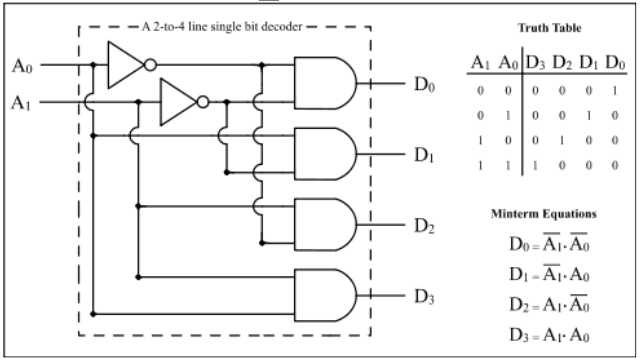
\includegraphics[width=0.8\textwidth]{images/Tema_3/Decodificador.PNG}
	\caption{Decodificador}
\end{figure}
\begin{figure}[H]
	\centering
	\lstinputlisting[style=customVHDL,  xleftmargin=.2\textwidth, xrightmargin=.2\textwidth]{Code/Tema_3/Decodificador.vhd}
	\caption{Código Codificador}
\end{figure}

\subsection{Decodificador}
\begin{figure}[H]
	\centering
	\lstinputlisting[style=customVHDL,  xleftmargin=.2\textwidth, xrightmargin=.2\textwidth]{Code/Tema_3/Codificador.vhd}
	\caption{Código Decodificador}
\end{figure}

\subsection{Multiplexor}

Descripción de alto nivel:
\[
	y = x_{s} \; donde \; s=\sum^{n-1}_{j=0} x_{j}2^{j}
\]

Implementación
\begin{itemize}
	\item 2 a 1 $y = x_{0} * \overline{s} + x_{1} * s$
	\item 4 a 1 $y = x_{0}\,\overline{s_{1}}\,\overline{s_{0}} + x_{1}\,\overline{s_{1}} \,s_{0} + x_{2}\,s_{1}\,\overline{s_{0}} + x_{3}\,s_{1}\,s_{0}$
\end{itemize}

\begin{figure}[H]
	\centering
	\lstinputlisting[style=customVHDL,  xleftmargin=.2\textwidth, xrightmargin=.2\textwidth]{Code/Tema_3/Multiplexor.vhd}
	\caption{Multiplexor}
\end{figure}
\newpage
\subsection{Sumador}
\begin{multicols}{2}
	\begin{figure}[H]
		\centering
		\lstinputlisting[style=customvhdl]{Code/Tema_3/Sumador1.vhd}
		\caption{Sumador con std\_logic}
	\end{figure}
	\vfill
	\null
	\begin{figure}[H]
		\centering
		\lstinputlisting[style=customvhdl]{Code/Tema_3/Sumador2.vhd}
		\caption{Sumador con numeric y datos con signo}
	\end{figure}
\end{multicols}

\begin{figure}[H]
	\centering
	\lstinputlisting[style=customvhdl]{Code/Tema_3/Restador.vhd}
	\caption{Restador}
\end{figure}


\section{Aritmética en VHDL}
\subsection{Operadores incluidos en VHDL-93 sin incluir ningún paquete}

\begin{table}[H]
	\begin{tabular}{|c|c|c|c|c|}
		\hline
		\rowcolor{gray}
		Operador & Descripción       & Tipo de operando a                          & Tipo de operando B                 & Tipo del resultado                 \\
		\hline
		a ** b   & Exponenciación    & Integer / Natural                           & Integer/ Natural                   & Integer / Natural                  \\
		\hline
		a * b    & Multiplicación    & \multirow{4}{*}{Integer / Natural}          & \multirow{4}{*}{Integer / Natural} & \multirow{4}{*}{Integer / Natural} \\
		\cline{1-2}
		a / b    & División          &                                             &                                    &                                    \\
		\cline{1-2}
		a mod b  & Módulo            &                                             &                                    &                                    \\
		\cline{1-2}
		a rem b  & Resto             &                                             &                                    &                                    \\
		\hline
		+ a      & Identidad         & \multirow{2}{*}{Integer / Natural}          &                                    & \multirow{2}{*}{Integer / Natural} \\
		\cline{1-2}
		- a      & Negación          &                                             &                                    &                                    \\
		\hline
		a + b    & Sumador           & \multirow{2}{*}{Integer / Natural}          & \multirow{2}{*}{Integer / Natural} & \multirow{2}{*}{Integer / Natural} \\
		\cline{1-2}
		a - b    & Resta             &                                             &                                    &                                    \\
		\hline
		a + b    & Concatenación     & Array 1-D, elemento                         & Array 1-D, elemento                & Array 1-D                          \\
		\hline
		a = b    & Igual             & \multirow{2}{*}{Cualquiera}                 & \multirow{2}{*}{Mismo que a}       & \multirow{2}{*}{boolean}           \\
		\cline{1-2}
		a /= b   & No igual          &                                             &                                    &                                    \\
		\hline
		a sll b  & Desp. Lóg. Izq.   & \multirow{6}{*}{bit\_vector}                & \multirow{6}{*}{Integer / Natural} & \multirow{6}{*}{bit\_vector}       \\
		\cline{1-2}
		a srl b  & Desp. Lóg. Der.   &                                             &                                    &                                    \\
		\cline{1-2}
		a sla b  & Desp. Arit. Der.  &                                             &                                    &                                    \\
		\cline{1-2}
		a sra b  & Desp. Arit. Der.  &                                             &                                    &                                    \\
		\cline{1-2}
		a rol b  & Rotación Izq.     &                                             &                                    &                                    \\
		\cline{1-2}
		a ror b  & Rotación der.     &                                             &                                    &                                    \\
		\hline
		a < b    & Menor que         & \multirow{4}{*}{Escalar o Array de 1-D}     & \multirow{4}{*}{Mismo que a}       & \multirow{4}{*}{boolean}           \\
		\cline{1-2}
		a <= b   & Menor o igual     &                                             &                                    &                                    \\
		\cline{1-2}
		a > b    & Mayor que         &                                             &                                    &                                    \\
		\cline{1-2}
		a >= b   & Mayor o igual que &                                             &                                    &                                    \\
		\hline
		a and b  & and               & \multirow{6}{*}{boolean, bit o bit\_vector} & \multirow{6}{*}{Mismo que a}       & \multirow{6}{*}{Mismo que a}       \\
		\cline{1-2}
		a or b   & or                &                                             &                                    &                                    \\
		\cline{1-2}
		a xor b  & xor               &                                             &                                    &                                    \\
		\cline{1-2}
		a nand b & nand              &                                             &                                    &                                    \\
		\cline{1-2}
		a nor b  & nor               &                                             &                                    &                                    \\
		\cline{1-2}
		a xnor b & xnor              &                                             &                                    &                                    \\
		\hline
	\end{tabular}
\end{table}

\subsection{Operadores y funciones del paquete IEEE std\_logic\_1164}
\begin{table}[H]
	\begin{tabular}{|c|c|c|c|}
		\hline
		\rowcolor{gray}
		Operador & Tipo de operando a                              & Tipo de operando b           & Tipo del resultado           \\
		\hline
		not a    & std\_logic\_vector, std\_logic                  &                              & Mismo que a                  \\
		\hline
		a and b  & \multirow{6}{*}{std\_logic\_vector, std\_logic} & \multirow{6}{*}{Mismo que a} & \multirow{6}{*}{Mismo que a} \\
		\cline{1-1}
		a or b   &                                                 &                              &                              \\
		\cline{1-1}
		a xor b  &                                                 &                              &                              \\
		\cline{1-1}
		a nand b &                                                 &                              &                              \\
		\cline{1-1}
		a nor b  &                                                 &                              &                              \\
		\cline{1-1}
		a xnor b &                                                 &                              &                              \\
		\hline
	\end{tabular}
\end{table}

\begin{table}[H]
	\begin{tabular}{|c|c|c|}
		\hline
		\rowcolor{gray}
		Función               & Tipo de operando a & Tipo de resultado \\
		\hline
		to\_bit(a)            & std\_logic         & bit               \\
		\hline
		to\_stdulogic(a)      & bit                & std\_logic        \\
		\hline
		to\_bitvector(a)      & std\_logic\_vector & bit\_vector       \\
		\hline
		to\_stdlogicvector(a) & bit\_vector        & std\_logi\_vector \\
		\hline
	\end{tabular}
\end{table}

\subsection{Operadores del paquete IEEE numeric\_std}
\begin{table}[H]
	\begin{tabular}{|c|c|c|c|}
		\hline
		\rowcolor{gray}
		Operador           & Tipo de operando a                                  & Tipo de operando b                                  & Tipo de resultado                 \\
		\hline
		abs a \newline - a & signed                                              &                                                     & signed                            \\
		\hline
		a * b              & \multirow{6}{*}{unsigned, natural, signed, integer} & \multirow{6}{*}{unsigned, natural, signed, integer} & \multirow{6}{*}{unsigned, signed} \\
		\cline{1-1}
		a / b              &                                                     &                                                     &                                   \\
		\cline{1-1}
		a mod b            &                                                     &                                                     &                                   \\
		\cline{1-1}
		a rem b            &                                                     &                                                     &                                   \\
		\cline{1-1}
		a + b              &                                                     &                                                     &                                   \\
		\cline{1-1}
		a - b              &                                                     &                                                     &                                   \\
		\hline
		a = b              & \multirow{6}{*}{unsigned, natural, signed, integer} & \multirow{6}{*}{unsigned, natural, signed, integer} & \multirow{6}{*}{boolean}          \\
		\cline{1-1}
		a /= b             &                                                     &                                                     &                                   \\
		\cline{1-1}
		a < b              &                                                     &                                                     &                                   \\
		\cline{1-1}
		a <= b             &                                                     &                                                     &                                   \\
		\cline{1-1}
		a > b              &                                                     &                                                     &                                   \\
		\cline{1-1}
		a >= b             &                                                     &                                                     &                                   \\
		\hline
	\end{tabular}
\end{table}

\subsection{Funciones de conversión de datos o casting}
Para la conversión de señales de un tipo a otro se deben usar las siguientes funciones y operaciones de casting:

\begin{figure}[H]
	\centering
	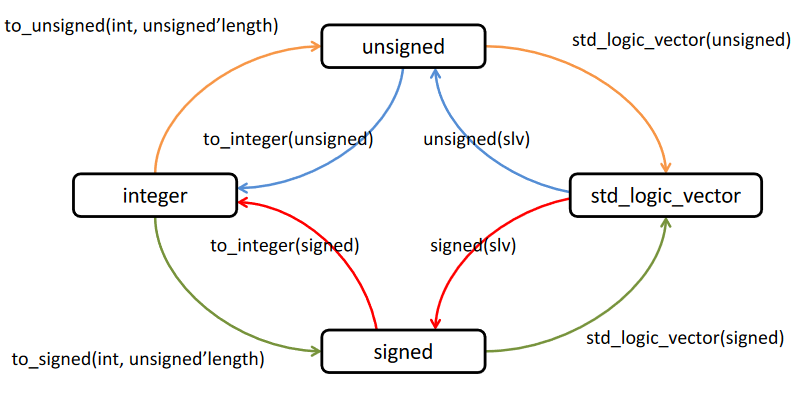
\includegraphics[width=0.9\textwidth]{images/Tema_3/casting.PNG}
	\caption{Funciones de conversión de tipos}
\end{figure}
\section{Unidades funcionales multifunción}
En este apartado se estudia la estructura del diseño y reducir la cantidad de recursos \gls{hw} compartiendo lógica entre distintas operaciones.\\
Para ello agruparemos \gls{uf} sencillas en \gls{uf} más complejas, esto se conoce como \gls{uf} multifunción. Esto lo utilizaremos cuando la \gls{uf} multifunción y el coste de conexión es menor que el coste de las \gls{uf} sencillas. Para lograr esto utilizaremos un algoritmo de particionamiento y un grafo de compatibilidad.
\begin{figure}[H]
	\centering
	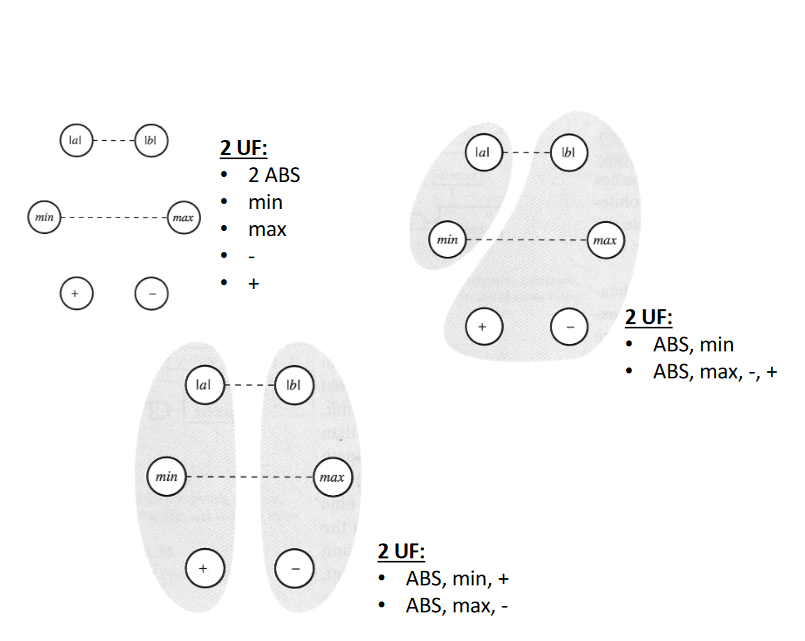
\includegraphics[width=0.5\textwidth]{images/Tema_3/Optimizacion.PNG}
	\caption{Optimización de múltiples \gls{uf}}
\end{figure}

\section{Redes iterativas}
Las redes iterativas son conjuntos de módulos idénticos, cada uno conectado exclusivamente a los módulos vecinos.

Una red iterativa 1-D de orden k es una implementación de una función de n variables, donde:
\begin{itemize}
	\item (n/k) celdas idénticas, G, con:
	      \begin{itemize}
		      \item Entradas externas x, e internas c
		      \item Salidas externas z, e internas c
	      \end{itemize}
	      \[
		      C_{j+1}=G\left(x_{j},c_{j}\right)
	      \]
	      \[
		      Z_{j}=F\left(x_{j}, c_{j}\right)
	      \]

	\item Celdas de los extremos pueden simplificarse aprovechando las condiciones de contorno
	      \begin{figure}[H]
		      \centering
		      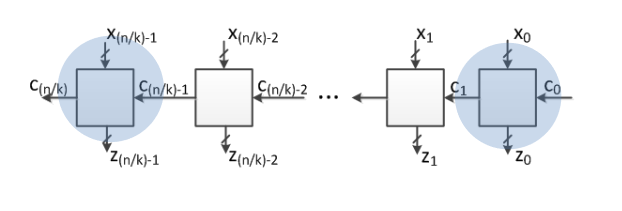
\includegraphics[width=0.6\textwidth]{images/Tema_3/Ejemplo_RI.PNG}
		      \caption{Ejemplo Red Iterativa 1-D}
	      \end{figure}
\end{itemize}

\subsection{Diseño}
Primero determinamos el valor de k, el equilibrio entre la complejidad de las celdas (nº de entradas) y el nº de celdas (retardo total).\\
Después determinamos los valores que deben trasmitirse entre los módulos intermedios (salidas internas) y el valor de la salida externa del último módulo. \\
Finalmente hacemos la descripción de alto nivel de los bloques intermedios, la implementación de las funciones de conmutación de los bloques, y la simplificación de las celdas inicial y final.

\subsection{Temporización}
Retardo $\left(\Delta\right)$
\begin{itemize}
	\item Función de retardo de las salidas externas de cada celda $\Delta_{o}$
	\item Función de retardo de las salidas internas de cada celda $\Delta_{c}$
\end{itemize}
\[
	\Delta = \left(\frac{n}{k}-1\right)\Delta_{c}+max\left(\Delta_{o}, \Delta_{c}\right)
\]

\subsection{Redes 1-D en VHDL}
En este ejemplo se diseñará una red de resolución de propiedades iterativa con n entradas y n salidas. LA salida $Z_{i} = 1\; si\; X_{i}= 1\; y\; X_{j} \forall j>i$

\begin{multicols}{2}
	\begin{figure}[H]
		\centering
		\lstinputlisting[style=customVHDL]{Code/Tema_3/Ejemplo_Celda_1.vhd}
		\caption{Ejemplo de celda de la red}
	\end{figure}
	\vfill
	\null
	\begin{figure}[H]
		\centering
		\lstinputlisting[style=customVHDL]{Code/Tema_3/Ejemplo_Array_Celdas_1.vhd}
		\caption{Generador de celdas conectadas}
	\end{figure}
\end{multicols}
\begin{figure}[H]
	\centering
	\lstinputlisting[style=customVHDL]{Code/Tema_3/Ejemplo_Red_1.vhd}
	\caption{Ejemplo red iterativa con generate}
\end{figure}

\subsection{Redes iterativas 2-D}
Array de celdas idénticas conectadas con sus vecinas. Cada celda (i,j) posee:
\begin{figure}[H]
	\centering
	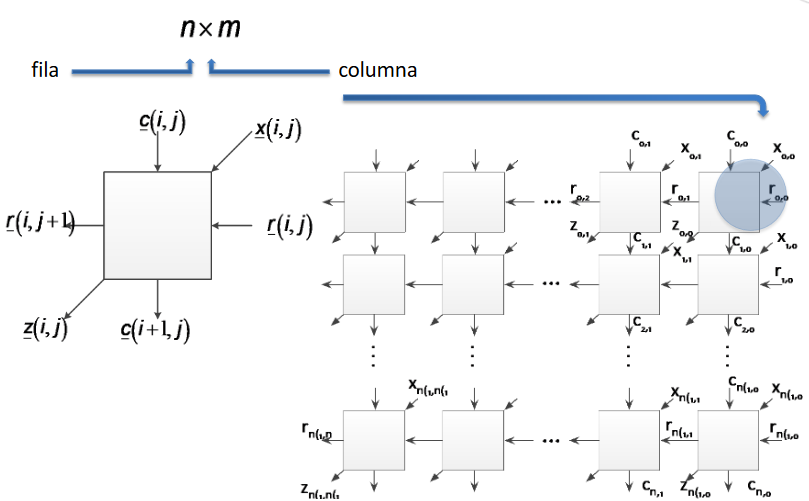
\includegraphics[width=\textwidth]{images/Tema_3/Red_2D.PNG}
\end{figure}

Para generar una matriz 2D tendremos que usar dos bucles anidados.

\section{Técnicas de mejora del rendimiento}
La utilización de diseños combinacionales bastante grandes (datos de entrada a partir de 32 bits), hace que el tiempo asociado al cambio crítico sea grande y el retardo de la red elevado.\\
En las redes iterativas la última celda no podrá generar su salida hasta que no haya recibido su señal intermedia. Esta señal interna ha tenido que atravesar n - 1 celdas que componen la red, por lo tanto el retardo es muy elevado si n es grande.

\subsection{Redes de anticipación}
Para reducir el retardo de las redes iterativas, anticiparemos el valor de la señal que se propaga entre celdas.

\begin{figure}[H]
	\centering
	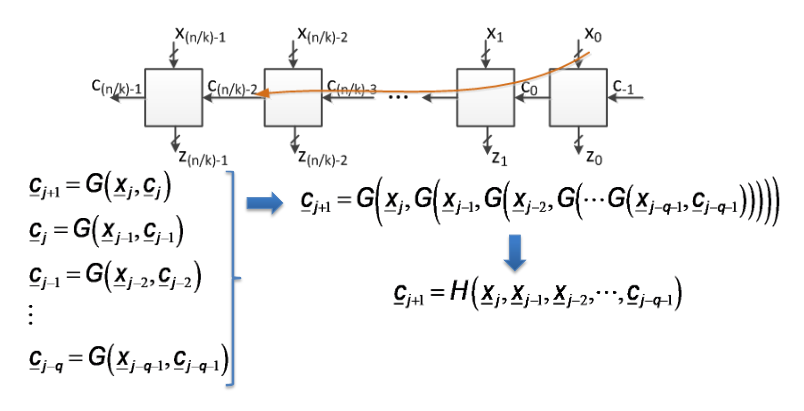
\includegraphics[width=\textwidth]{images/Tema_3/Redes_Anticipacion_1.PNG}
	\caption{Red iterativa sin anticipación}
\end{figure}
\begin{figure}[H]
	\centering
	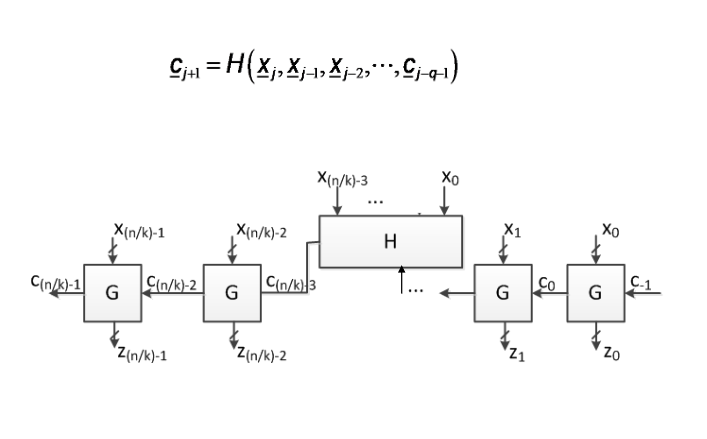
\includegraphics[width=\textwidth]{images/Tema_3/Redes_Anticipacion_2.PNG}
	\caption{Red iterativa con anticipación}
\end{figure}
\newpage
\subsection{Redes en árbol}
Implementar una función de n entradas usando bloques de k entradas:
\begin{figure}[H]
	\centering
	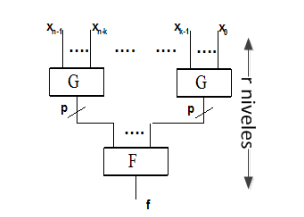
\includegraphics[width=0.5\textwidth]{images/Tema_3/Red_Arbol.PNG}
	\caption{Red en árbol}
\end{figure}
\begin{itemize}
	\item Módulo G: k entradas y p salidas $\rightarrow \frac{n}{k}$ módulos
	\item Módulo F: $p\frac{n}{k}$ entradas
	\item Retardo: $\left(r - 1\right)\Delta_{G} + \Delta_{F}$
\end{itemize}

\section{Errores de diseño}
\subsection{Lazos combinacionales}
Estructuras lógicas que contienen realimentación sin ningún elemento síncrono en el camino. Por ejemplo \textcolor{blue}{$A <= A + 1;$} \gls{vhdl} no permitirá ni la simulación ni la síntesis de este diseño.
\subsection{Errores de diseño en circuitos combinacionales}
Si implementamos la lógica combinacional mediante un process:
\begin{itemize}
	\item\textbf{Error 1:} no incluir todas las entradas en la lista de sensibilidad
	\item\textbf{Error 2:} no terminar una sentencia if con un else
	\item\textbf{Error 3:} no especificar el valor de alguna salida en alguna de las ramas de la sentencia if
\end{itemize}

En los errores 2 y 3 se añadirá un latch, lo que implica lógica secuencial.
